% \newcommand{\floor}[1]{\left\lfloor {#1} \right\rfloor}
% \newcommand{\unix}{{\tt UNIX}}
% \newcommand{\dos}{{\tt DOS}}
% \newcommand{\tildegen}{\protect\raisebox{-0.12cm}{\symbol{'176}}}

\section{Introduction}
\begin{verse}
``In the computer industry, there are three kinds of lies: lies, damn lies, and
 benchmarks.''
\end{verse}
This document describes a practical toolkit to evaluate the status of code. 
It can be used to create programs that measure performance, known as 
benchmarks, and other various tests, execute them, and analyze their results. 
With little effort a user of this toolkit can detect inefficiencies, 
bottlenecks, and loss of functionality or performance degradation, compare 
various techniques, algorithms, and different implementations, and measure 
progress. A user, can then, present the results in a comprehensible way. The 
information produced also includes the precise description of the execution 
environment to allow the reproduction of the results.

There are two directives that must be followed in order to write bug-free code.
The first is to prevent the introduction of bugs in the first place. The second
is to find bugs as soon as they are introduced. This toolkit can be used to
build a full blown automatic system for bug detection, also known as regression
tests. We haven't used the toolkit in such a way so far, but we may exploit
this option in the future.

The toolkit is designed as a independent component in a large-scale
development environment. Final products and intermediate products that
are required to build other products are installed into a dedicated
database referred as {\em ROOT}, and pointed to by the environment
variable {\tt \$ROOT}. While the toolkit assumes that certain files are
installed into {\em ROOT}, it allows you to redefine {\em ROOT's}
location and other pieces that are based on {\em ROOT's} location
through command-line options.

The toolkit consists of three parts that corresponds to the three phases
required to evaluate code; (i) The creation of a hierarchy of test or benchmark
programs, (ii) the selective and controlled execution of the programs with
various input test cases, and (iii) the analysis and profiling of their results
and the conversion of the data into more meaningful and comprehensible
presentations. The following Sections describe the three parts in details.

It must be noted that our goal here is not to replace existing tools
that already provide useful functionality for computational
experiments (e.g., gnuplot, make, perl, python). Rather, the goal is
to augment this set with new tools that build on the functionality
already available to provide a comfortable testing environment.

It's worth mentioning the \textbf{ExpLab} tool set for Computational
Experiments by Susan Hert, Lutz Kettner, Tobias Polzin, and Guido
Sch{\"a}fer from the Max-Planck-Institut f{\"u}r Informatik. There seems to be
little overlap between \textbf{ExpLab} and our toolkit, but for most
they emphasize different aspects.

\section{Creation}

The toolkit was developed as a package in \cgal, the Computational
Geometry Algorithms and Data Structures library, to aid in the
development and maintenance of the planar map modules. As a 
\cgal\ module on its own, it obliges to the Generic Programming Paradigm. 
The first part consists of a couple of generic C++ classes, and the
interface between them and the user code to be evaluated. Some of the code 
and documentation is derived from the material developed in the 
\textsc{Acs} project, parts of which are published in \cite{cgal:f-ecsca-04}.

The \ccc{Bench_option_parser} class is used to parse command line options, 
interpret them, and configure the bench accordingly. The benchmark itself 
is performed through the \textbf{()} operator of the \ccc{Bench} class 
described next.

The \ccc{Bench} class is parameterized with a model of the
{\em Benchable} concept. This concept serves as the interface between
the measuring device and the operation you wish to measure, refereed
as the target operation here after. A model of this concept must
satisfy a few requirements as follows. It must have a default
constructor, and it must provide four methods. The
\ccc{init()} method can be used to initialize some data
members before the target operation is carried out. The
\ccc{clean()} method is used to clean those data members
and residual data of the operation after the measure is completed. The
\ccc{sync()} method can be used to synchronize between the
target operation and the time-sampling operations. While these three
methods must be provided, they can be empty. The \ccc{op()}
method performs the target operation. This operation is executed in a
controlled loop according to various criteria explained in the next
paragraph.

If the estimated time-duration it takes to complete a single execution
of the target operation is large compared to the granularity of the
timing device, it is sufficient to execute the target operation a
small number of times between sampling the timing device, perhaps even
once. You can set the number of times the target operation is executed
through the \ccc{set_samples()} interface method of the
\ccc{Bench} class. On the other hand, if the estimated
time-duration of a single execution is of the same order as the
granularity of the timing device, increasing the number of executions
increases the accuracy of the measure. With the
\ccc{set_seconds()} method of the \ccc{Bench}
class, you can set the time slot in seconds allocated for the
measure. In this case the target operation is executed in a loop while
the number of executions is counted. When the time expires, the
counter is sampled. Then, the target operation is executed again for
as many times as counted, while measuring the time it takes to
complete the sequence.

\subsection*{A simple Benchmark Program}
The basic structure of a useful benchmark program can be very simple; Its
tasks are to measure the time it takes to complete a sequence of
executions of the target operation, and present the results in some useful
manner.

Below you can find the listing of a program that measures the time it takes
to compute the square root of $\Pi$, and produces the results shown in figure 
\ref{sqrtResults}

\begin{figure}[!hbp]
\begin{verbatim}
Bench                            Bench    Ops      Total    Single   Num Ops
    Name                             Time      Num Ops Time  Op Time  Per Sec
-------------------------------- -------- -------- -------- -------- --------
Square root                             1 14690512   1.0000   0.0000 14690512.0000
\end{verbatim}
\caption{Square-root benchmark results.}\label{sqrtResults}
\end{figure}

The \textbf{()} operator of the \ccc{Bench} class counts the number
of times the function \textbf{sqrt()} can be executed within the allocated time
slot. Then, it executes the \ccc{sqrt()} function for as many times as
counted, while measuring the time it takes to complete the sequence.

By default the allocated time slot is 1 second. The program overrides the
default with the number of seconds returned by the
\ccc{get_seconds()} method of the
\ccc{Bench_option_parser} class. The default of the later is
1 second as well, and can be overridden with the \textbf{``-t {\em seconds}''}
command-line option.

\ccIncludeExampleCode{../examples/Benchmark/simple.cpp}

\section{Bnechmark File Format}
We present a common file format for data instances and for benchmarking 
\cgal\ software. It supports benchmarks on algebraic data as well as curve 
and surface data. We document the file format grammar, a reference parser 
implementation, and how it can be extended.
It is derived from the material developed in the \textsc{Acs} project.

% +------------------------------------------------------------------------+
% | Reference manual page: Convex_hull_d_ref/intro.tex
% +------------------------------------------------------------------------+

%\clearpage
%\section{Reference Pages for dD Convex Hulls and Delaunay Triangulations}
\ccRefChapter{dD Convex Hulls and Delaunay Triangulations\label{chap:convex_hull_d_ref}}
\ccChapterAuthor{Susan Hert \and Michael Seel}

A subset $S \subseteq \R^3$ is convex if for any two points $p$ and $q$
in the set the line segment with endpoints $p$ and $q$ is contained
in $S$. The convex hull\ccIndexMainItemDef{convex hull} of a set $S$ is 
the smallest convex set containing
$S$. The convex hull of a set of points $P$ is a convex 
polytope with vertices in $P$.  A point in $P$ is an extreme point 
(with respect to $P$)\ccIndexMainItemDef{extreme point} if it is a vertex 
of the convex hull of $P$.

\cgal\ provides functions for computing convex hulls in two, three 
and arbitrary dimensions as well as functions for testing if a given set of 
points in is strongly convex or not.  This chapter describes the class
available for arbitrary dimensions and its companion class for 
computing the nearest and furthest side Delaunay triangulation. 

\section{Classified Reference Pages}

\ccHeading{Concepts}

\ccRefConceptPage{ConvexHullTraits_d} \\
\ccRefConceptPage{DelaunayLiftedTraits_d} \\
\ccRefConceptPage{DelaunayTraits_d} \\

\ccHeading{Classes}

\ccRefIdfierPage{CGAL::Convex_hull_d_traits_3<R>} \\
\ccRefIdfierPage{CGAL::Convex_hull_d<R>}  \\
\ccRefIdfierPage{CGAL::Delaunay_d< R, Lifted_R >} 

\clearpage



% ---------------------------------------------------------------------------
\subsection{Benchmark File Format}

We use plain \ascii\ text files for our format. The actual structure
of the file is not important for the interpretation. In principal, the
file could be written in a single line (with the exception of
comments, see below). For the potential human reader, a sensible
layout and a restriction to eighty columns are helpful. The definition
of terminal symbols and handling of comments and white spaces is
explained in Section~\ref{lexer}. Include files are explained in
Section~\ref{inclfiles}. 

In the following we format \ts{terminal symbols} in
\ts{typewriter} font and \nts{non-terminal symbols} in \nts{boldface}.
Grammar rules for non-terminal symbols are occasionally given in the
extended Backus Naur Form (EBNF), where \texttt{::=} has the meaning
of ``is defined as'', \texttt{|} separates two alternative choices,
\texttt{[]} encloses an optional part, and \verb|{}| encloses a
repetitive part (zero or more times).

The grammar and its reference parser implementation support the
feature to read a sequence of several benchmark files, for example,
concatenated together.  A benchmark file consists of four parts; a
magic token identifying the file format, a sequence of file header
options, a sequence of classifications, and a sequence of the objects
that define the benchmark content, e.g., polynomials, curves, or
surfaces. These sequences might be empty. Formally:
\medskip

\begin{tabular}{lll@{\hspace{10mm}\ldots\ }l}
%  \nts{Input} & \ts{::=} & \multicolumn{2}{l}{\Open\ \nts{File} \Close}\\[\ebnfskip]
  \nts{Input} & \ts{::=} & \multicolumn{2}{l}{\nts{File}}\\[\ebnfskip]
  \nts{File}  & \ts{::=} & \nts{FileFormat} & see Section~\ref{headerformat}\\
              &          & \verb|{| \nts{FileHeaderOption} \verb|}| 
                                          & see Section~\ref{headeropt}\\
              &          & \verb|{| \nts{Classification} \verb|}|
                                          & see Section~\ref{classification}\\
              &          & \verb|{| \nts{Object} \verb|}|
                                          & see Section~\ref{grammar}
\end{tabular}

We give a short example file that contains a single line segments. The
end points are given with homogeneous integer coordinates. A longer
example can be found in Section~\ref{longexample}.

\begin{verbatim}
# simple example with one random line segment
FileFormat( "AcsBenchmark", 0, 1 )
BenchmarkName( "Lines" ) 
Classification( "Arrangement", "Lines", "BoundedArcs", "Rnd", "2", "Sept-2004")
LineSegment_2( Point_2(1,1,1), Point_2(8,5,2))
\end{verbatim}

\subsection{Lexer Tokens, Comments, and White Spaces}
\label{lexer}

A \verb|#| character starts a single-line comment up to the end of the
current line. 

\begin{alltt}
\ts{#} commentary text, or
Conic(1,2,3,4,5,6) \ts{#} commentary text until the end of the line
\end{alltt}

\noindent
Longer and also possibly nested comments stretching over multiple
lines can be enclosed with the keyword \ts{Comment(...)}, however,
parenthesis must match up properly:

\begin{alltt}
\ts{Comment(} commentary text (even nested)
         across multiple lines \ts{)}
\end{alltt}

\noindent
Comments and white spaces can be used everywhere in the file and are
ignored by the parser.

The lexical analyzer (lexer) detects all terminal symbols. Besides the
keywords, such as \ts{Comment}, these are numbers, strings, and the
constants \ts{VOID}, \ts{MINUS\_INFTY}, \ts{PLUS\_INFTY},
\ts{COUNTERCLOCKWISE}, and \ts{CLOCKWISE}. In particular we have:
\medskip

\begin{tabular}{ll}
  \ts{INTEGER} &  integer number of arbitrary precision, may have a
  leading sign.\\[\ebnfskip]
  \ts{FNUMBER} &  floating point number in the usual scientific
  notation, but not an \ts{INTEGER}, \\ & and restricted to IEEE double
  precision. \\[\ebnfskip]
  \ts{STRING}  &  string in double quotes \ts{"..."}, may include
  newlines. The escape character \verb|\| \\ & can be used to represent
  double quotes within the string as \verb|\"|, or to represent\\ & the
  escape character itself in the string as \verb|\\|.
\end{tabular}

\subsubsection{IncludeFile}
\label{inclfiles}

The file format and the reference parser implementation support
include files. They are not used in the current plans for benchmarks,
but they might turn out to be useful later for the hierarchical data
sets. A statement \ts{IncludeFile(}\textit{filename}\ts{)} instructs
the lexical scanner to stop scanning the current file and to continue scanning
the new file with the given \textit{filename}. Once the end of new
file has been reached, scanning resumes in the old file right after
the include statement. Include statements can be nested to an
arbitrary depth. An example:

\begin{verbatim}
IncludeFile( FullConicsRnd_10_1.arr)
\end{verbatim}

\subsubsection{FileFormat}
\label{headerformat}

The mandatory \ts{FileFormat} field contains the \emph{magic-key\/}
string ``AcsBenchmark'' such that the parser recognizes that this file
is supposed to be a valid benchmark file.  The field also contains a
major and a minor version number. If the minor version number changes,
the parser with the same (or higher) major version number can still
process the file. If the major version number of the file is higher
than the major version number of the parser (fundamental modifications
in the format definition were made), the parser cannot read the format
any longer and throws an exception. An example:

\begin{verbatim}
FileFormat( "AcsBenchmark", 0, 1 )
\end{verbatim}

\subsubsection{FileHeaderOption}
\label{headeropt}

Currently, only one file header option is specified, the
\ts{BenchmarkName}. It corresponds to the filename and reflects part
of the classification, see Section~\ref{classification}. One benefit
is that already the filename communicates the types of objects, how
many there are, which random number seed has been used, and if the
objects are randomized or degenerated. Grammar:

\medskip
\begin{tabular}{lll}
  \nts{FileHeaderOption} & \ts{::=} & \ts{BenchmarkName( STRING )}
\end{tabular}

\subsubsection {The Classification}
\label{classification}

The classification declares what types of objects appear in the
benchmark file. The classification is inspired by hierarchical
biological classifications. It consists of a sequence of string
arguments that go from the general to the specific properties of a
benchmark. Thus, the classification is subject to additions whenever a
new benchmark is devised. In particular, the number of properties
might not be the same for all classifications. However currently it
consists of six properties.  Note that such a tree-shaped
classification is not necessarily the only valid view on such a
classification problem, e.g., which property is more specific than
some other property. We also allow property entries to be undefined
and set to the empty string \ts{""}.
The classification with its dependencies is illustrated in
Figure~\ref{bench_fig::class}.

\begin{figure}[t]
\begin{ccTexOnly}
  \begin{center}
  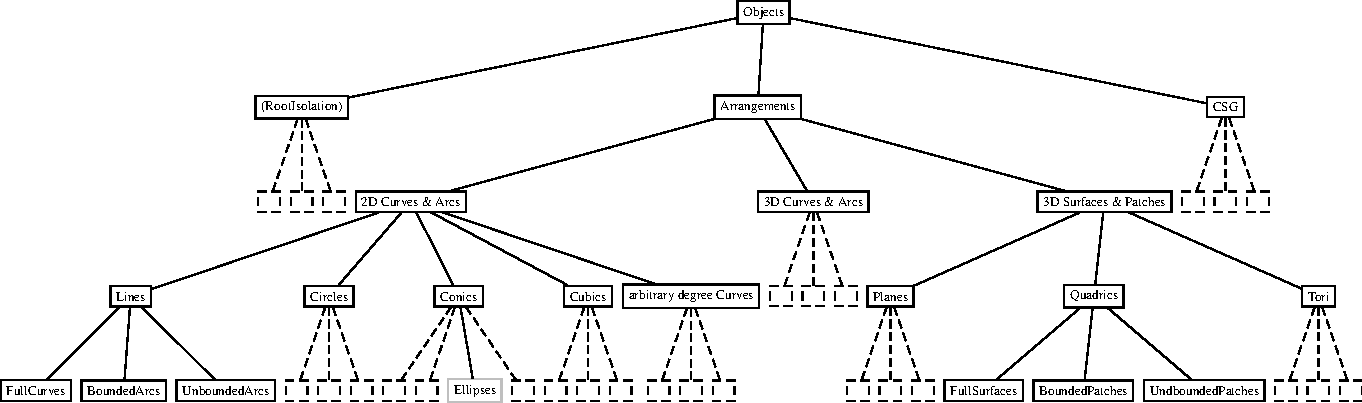
\includegraphics[width=\textwidth]{Benchmark/fig/classification}
  \end{center}
\end{ccTexOnly}
\begin{ccHtmlOnly}
  <p><center>
  <img src="./fig/classification.gif" border=0 alt="classification">
  </center>
\end{ccHtmlOnly}
\caption{Classification\label{bench_fig::class}}
\end{figure}

\begin{itemize}
  \item {\bf Problem:} the algorithmic problem that this benchmark
    addresses. Possible choices are \ts{"Arrangement"} for arrangement
    computations or \ts{"CSG"} for a constructive solid
    geometry Boolean operations evaluation problem. The filename
    suffix  depends on the problem. It is \ts{.arr} or \ts{.csg}
    correspondingly. Once ACS project members see further demands, 
    it can be easily extended.
  \item {\bf Geometry:} distinguishes between the 2D and 3D supporting
    geometric objects. In 2D the choices are \ts{"Lines"},
    \ts{"Circles"}, \ts{"Conics"}, \ts{"Cubics"}, \ts{"Quartics"}, and
    \ts{"arbitrary degree curves"}. In 3D the choices are 
    \ts{"Planes"}, \ts{"Quadrics"}, and \ts{"Tori"}.
  \item {\bf Class:} In 2D the choices are \ts{"FullCurves"},
    \ts{"BoundedArcs"}, and \ts{"UnboundedArcs"}, where unbounded arcs
    obviously also cover bounded arcs. For conics the class could
    additional be set to \ts{"Ellipses"}. In 3D the choices are
    \ts{"FullSurfaces"}, \ts{"BoundedPatches"}, and \ts{"UnboundedPatches"}. 
  \item {\bf Family:} specifies the specific property that
    characterizes this specific set of benchmark objects. For example,
    families of random objects are named \ts{"Rnd"} and families of
    degenerate objects are named \ts{"Dgn"}. 
  \item {\bf Instance:} extends the family to specific collection of
    benchmark object, for example, for a family of random objects by
    fixing the seed of the pseudo random number generator (thus
    specifying a deterministic sample of the random distribution).
  \item {\bf Revision:} contains the latest date when the benchmark was
    specified or modified. These modifications are expected to be
    infrequent, so we store just the month and year, such as in
    \ts{"May-2005"}. 
\end{itemize}

\noindent
The filename consists of the concatenation of the \nts{Geometry}, the
\nts{Class}, the \nts{Family}, the number of objects in the file, the
\nts{Instance}, and the suffix according to the \nts{Problem}.

Here is an example for a complete Classification:

% ??????
%Classification("Arrangement", "Conics", "FullCurves", "FullConicsRnd_30", 
%               "FullConicsRnd_30_2", "May-2005")

\begin{verbatim}
Classification("Arrangement", "Conics", "FullCurves", "Rnd", "2", "May-2005")
\end{verbatim}

\noindent
This classification example describes a benchmark file which contains
a sequence of random conics generated starting with a pseudo random
number generator seed 2. Assuming we have thirty conics in this file
then we get its corresponding filename as
\texttt{ConicsFullCurvesRnd\_30\_2.arr}. 
  
There can be more than one classification in a benchmark file, i.e., if
a single benchmark file contains a combination of different object types.
For example, a file containing circles, bounded conic arcs, and
ellipses, has the classification:

\begin{verbatim}
Classification("Arrangement", "Circles",  "FullCurves", "Rnd", "2", "May-2005")
Classification("Arrangement", "Conics",  "BoundedArcs", "Rnd", "2", "May-2005")
Classification("Arrangement", "Ellipses", "FullCurves", "Rnd", "2", "May-2005")
\end{verbatim}

\noindent
The classification must contain an entry for each distinct object
type, such that an application can rely on the classification to the
extend that if the classification mentions only conics but not
circles then the file does not contain \ts{"Circle\_2"} entries. Or
the other way around, if the application does not wish to handle
circles, it can issue an error message as soon as it sees the
classification mentioning circles. Note that of course mathematically
a conic can represent a circle as well, but this will not require the
classification to mention circles.

Finding a good filename for such a combined file might become difficult.
However, assuming we have sixty curves and arcs in this file, we could
suggest for a corresponding filename
\texttt{CirclesEllipsesFullCurvesConicsBoundedArcsRnd\_60\_2.arr}, and
it simplifies matters if the seed values are the same. In principle,
the filename could be shortened to express only commonalities of the
objects if it does not create conflicts with other filenames. For
example, combined data sets are likely to come from a specific example
or application and could have a common instance name, such as
\ts{"CgalLogo"} for the \cgal\ logo that consists of full circles and
line segments. Its filename could be shortened to
\texttt{CirclesCgalLogo\_92.arr}.

Combining different problems or different dimensions in one file does
not seem to make sense from our current perspective.

% -------------------------------------------------------------------------
\subsubsection{File Format for Individual Objects\label{grammar}}

We describe the individual objects in the following table. The first
column lists the non-terminal symbol. The second column lists grammar
rules where several alternative choices are listed below each other.
The third column gives a description of the object.  Non-terminal
symbols formatted in boldface are valid \nts{Object} entries that can
follow the classification. The other non-boldface non-terminal symbols
are only used within the grammar rules of other symbols.  The non-bold
objects are auxiliary tokens that occur only in the structure of bold
objects. \medskip

\begin{ccTexOnly}
\begin{tabular}{*{3}{| l} |} \hline
Object   & syntax                         & description \\ \hline \hline
Integer  & INTEGER                        & an integer value \\ \hline
Rational & Rational (Integer, Integer)    & Rational(integer nominator, \\
         &                                & \ \ \ \ \ \ \ \ \ \ \ \ \ integer denominator)
                                            \\ \hline
Infty    & MINUS\_INFTY                   & encodes $-\infty$ \\ 
         & PLUS\_INFTY                    & encodes $+\infty$  \\ \hline

Integer\_sequence & Integer, Integer ...
                        & a sequence of arbitrary many integer  \\ 
                  &     &  values \\ \hline
Monom & (Integer, (Integer\_sequence)) & monom with integer coefficient and exponent sequence, \\
      &                                & starting with the first variable \\ \hline
Monom\_sequence & Monom, Monom ... & a sequence of arbitrary many monoms \\ \hline
%Integer\_sequence\_2 & integer\_sequence\_2(
%                       & a sequence of an even number of \\
%                  & \ \ Integer, Integer, ... ) & integer values\\ \hline
Orientation & COUNTERCLOCKWISE            & orientation of a ConicArc  \\
            & CLOCKWISE                   &           \\
            & VOID                        &           \\ \hline

Point\_2 & Point\_2 (Integer,Integer)     & cartesian point with \\
         &                                & \ \ integer coordinates x and y \\
         & Point\_2 (Integer,Integer,Integer) & homogeneous point with \\ 
         &                                & \ \ integer coordinates x,y,w\\
         & Point\_2 (Rational,Rational)   & cartesian point of two \\
         &                                & \ \ rational coordinates x,y\\ \hline
%InterpolationPoint & InterpolationPoint\_2 (   & an InterpolationPoint consits 
%                                                  of a point \\
%                   & \ \ Point\_2 ,            & and its derivations\\
%                   & \ \ Integer\_sequence\_2 )&  \\ \hline
{\bf Polynomial}    & {\bf Polynomial\_1} (Integer\_sequence) 
                             & the coefficients of an integer polynomial \\ \hline
                    & {\bf Polynomial} $<n>$ (Monom\_list)
                             & the monoms of a $n$-variate polynomial \\ \hline

AlgebraicReal & AlgebraicReal (         & an algebraic real is a real root\\
              & \ \ Polynomial,         & of a polynomial defined by an\\
              & \ \ Rational,Rational,  & isolating interval with rational boundaries\\
              & \ \ Integer)            & or redundantly by the index of the root\\ \hline

{\bf LineSegment} & {\bf LineSegment\_2} (Point\_2,Point\_2) & LineSegment\_2 (source, target) \\ \hline

{\bf Circle}   & {\bf Circle\_2} (Point\_2,Integer) & Circle\_2 (center, radius) \\ 
               & {\bf Circle\_2} (Point\_2,Rational) & Circle\_2 (center, radius) \\ \hline

{\bf Conic}  & {\bf Conic\_2} (
                               & Conic defined by its 6 coefficients \\
             & \ \ \ \ \ Integer,Integer,Integer,
                     &  (A,B,C,D,E,F) \\
             & \ \ \ \ \ Integer,Integer,Integer)        
                     &  \begin{math} Ax^2+Bxy+Cy^2+Dx+Ey+F \end{math}\\ \hline

%{\bf InterpolatedConic} & {\bf InterpolatedConic} (   
%                                            & consits of a nonempty sequence \\
%                 & \ \ Interpolation\_point\_2\_sequence ) 
%                                            & of InterpolationPoints\\ 
%                  &                         & 5 interpolation conditions 
%                                                    are necessary\\ 
%                  &                         & for a conic \\ \hline

ConicPoint    & ConicPoint\_2 (Conic,  
                        & ConicPoint (Conic, x-coordinate, \\
              & \ \ AlgebraicReal,Integer)  
                        & \ \ arc number implying y-coordinate (0 or 1)) \\
              & ConicPoint\_2 (Conic,          
                        & ConicPoint (Conic, x-coordinate at infinity, \\
              & \ \ infty,Integer) 
                        & \ \ arc number) \\
              & ConicPoint\_2 (Conic,    
                        & ConicPoint (Conic, x-coordinate, \\
              & \ \ AlgebraicReal,infty) 
                        & \ \ y-coordinate at infinity) \\ \hline
%              & ConicPoint\_2 (InterpolatedConic,  
%                       & ConicPoint (Conic, y-coordinate, \\
%              & \ \ AlgebraicReal, Integer)  
%                        & \ \ x-coordinate) \\
%              & ConicPoint\_2 (InterpolatedConic,    
%                      & ConicPoint (Conic, y-coordinate, \\
%              & \ \ AlgebraicReal, infty) 
%                    & \ \ x-coordinate) \\
%              & ConicPoint\_2 (InterpolatedConic,          
%                  & ConicPoint (Conic, y-coordinate, \\
%              & \ \ infty, Integer) & \ \ x-coordinate) \\ \hline



{\bf ConicArc}      & {\bf ConicArc\_2} (Conic,    & an Arc of a Conic \\
              & \ \ ConicPoint,                    & with source,\\
              & \ \ ConicPoint,                    & target, and\\
              & \ \ Orientation)                   & its orientation\\
%              & {\bf ConicArc\_2} ( InterpolatedConic,    & \\
%              & \ \ ConicPoint,                    & \\
%              & \ \ ConicPoint,                    & \\
%              & \ \ orientation)                   & \\               
              & {\bf ConicArc\_2} (ConicPoint)      & degenerated arc (single point) \\ \hline


{\bf Cubic} & {\bf Cubic\_2} (        & Cubic defined by its 10 coefficients \\
      & \ \ Integer, Integer, Integer & (A,B,C,D,E,F,G,H,K,L)\\
      & \ \ Integer, Integer, Integer & \begin{math} Ax^3+Bx^2y+Cxy^2+Dy^3+Ex^2+ \end{math}\\
      & \ \ Integer, Integer, Integer & \begin{math}Fxy+Gy^2+Hx+Ky+L\end{math}\\
      & \ \ Integer)                  & \\ \hline

%{\bf InterpolatedCubic} & {\bf InterpolatedCubic\_2} (   & \\
%                  & \ \  Interpolation\_point\_2\_sequence ) & \\ \hline
{\bf Quadric} & {\bf Quadric\_3} (      & Quadric defined by its 10 coefficients \\
        & \ \ Integer, Integer, Integer & (A,B,C,D,E,F,G,H,K,L)\\
        & \ \ Integer, Integer, Integer & \begin{math} Ax^2+Bxy+Cxz+Dy^2+Eyz+ \end{math}\\
        & \ \ Integer, Integer, Integer & \begin{math}Fz^2+Gx+Hy+Kz+L\end{math}\\
        & \ \ Integer)                  & \\ \hline
\end{tabular}
\end{ccTexOnly}

\begin{ccHtmlOnly}
<div align="center">
<table cellpadding=3 border="1">
<tr><th>Object</th><th>syntax</th><th>description</th></tr>
<tr><td>Integer</rd><td>INTEGER</td><td>an integer value</td></tr>
<tr><td>Rational</td><td>Rational (Integer, Integer)</td>
  <td>Rational(integer nominator, integer denominator)</td></tr>
<tr><td>Infty</td>
    <td>MINUS_INFTY<BR>
        PLUS_INFTY</td>
    <td>encodes $-\infty$<BR>
        encodes $+\infty$</td></tr>
<tr><td>Integer_sequence</td>
    <td>Integer, Integer ...</td>
    <td>a sequence of arbitrary many integer values</td></tr>
<tr><td>Monom</td>
    <td>(Integer,(Integer_sequence))</td>
    <td>coefficient(exponent_sequence)</td></tr>
<tr><td>Monom_sequence</td>
    <td>Monom, Monom ...</td>
    <td>a sequence of arbitrary many monoms</td></tr>
<tr><td>Orientation</td><td>COUNTERCLOCKWISE<br>CLOCKWISE<br>VOID</td><td>orientation of a ConicArc</td></tr>
<tr><td>Point_2</td>
  <td>Point_2 (Integer,Integer)<br>
      Point_2 (Integer,Integer,Integer)<br>
      Point_2 (Rational,Rational)</td>
  <td>cartesian point with integer coordinates x and y<br>
      homogeneous point with integer coordinates x,y,w<br>
      cartesian point of two rational coordinates x,y</td></tr>
<tr><td rowspan="2"><b>Polynomial</b></td>
    <td><b>Polynomial_1</b>(Integer_sequence)</td>
    <td>the coefficients of an integer polynomial</td></tr>
<tr><td><b>Polynomial</b>&lt;<i>n</i>&gt;(Monom_sequence)</td>
    <td>monoms of a <i>n</i>-variate polynomial</td></tr>
<tr><td>AlgebraicReal</td>
    <td>AlgebraicReal(Polynomial,Rational,Rational,Integer)</td>
    <td>an algebraic real is a real root of a polynomial defined by an
        isolating interval with rational boundaries or redundantly by
	the index of the root</td></tr>
<tr><td><b>LineSegment</b></td><td><b>LineSegment_2</b>(Point_2,Point_2)</td>
  <td>LineSegment_2(source, target)</td></tr>
<tr><td><b>Circle</b></td><td><b>Circle_2</b>(Point_2,Integer)<br>
                              <b>Circle_2</b>(Point_2,Rational)</td>
  <td>Circle_2(center, radius)<br>
      Circle_2(center, radius)</td></tr>
<tr><td><b>Conic</b></td>
  <td><b>Conic_2</b>(Integer,Integer,Integer,Integer,Integer,Integer)</td>
  <td>Conic defined by its 6 coefficients (A,B,C,D,E,F)<br>
      <i>Ax<sup>2</sup>+Bxy+Cy<sup>2</sup>+Dx+Ey+F</i></td></tr>
<tr><td>ConicPoint</td><td>ConicPoint_2(Conic,AlgebraicReal,Integer)<br>
                           ConicPoint_2(Conic,infty,Integer)<br>
			   ConicPoint_2(Conic,AlgebraicReal,infty)</td>
                       <td>ConicPoint(Conic, x-coordinate, arc number implying y-coordinate (0 or 1))<br>
		           ConicPoint(Conic, x-coordinate at infinity, arc number)<br>
                           ConicPoint(Conic, x-coordinate, y-coordinate at infinity)</td></tr>
<tr><td><b>ConicArc</b></td>
    <td><b>ConicArc_2</b>(Conic,ConicPoint,ConicPoint,Orientation)<br>
        <b>ConicArc_2</b>(ConicPoint)</td>
    <td>an Arc of a Conic with source, target, and its orientation<br>
        degenerated arc (single point)</td></tr>
<tr><td><b>Cubic</b></td>
    <td><b>Cubic_2</b>(Integer,Integer,Integer,Integer,Integer,<br>
                       Integer,Integer,Integer,Integer,Integer)</td>
    <td>Cubic defined by its 10 coefficients (A,B,C,D,E,F,G,H,K,L)<br>
        <i>Ax<sup>3</sup>+Bx<sup>2</sup>y+Cxy<sup>2</sup>+Dy<sup>3</sup>+Ex<sup>2</sup>+Fxy+Gy<sup>2</sup>+Hx+Ky+L</i></td></tr>
<tr><td><b>Quadric</b></td>
    <td><b>Quadric_3</b>(Integer,Integer,Integer,Integer,Integer,<br>
                         Integer,Integer,Integer,Integer,Integer)</td>
    <td>Quadric defined by its 10 coefficients (A,B,C,D,E,F,G,H,K,L)<br>
        <i>Ax<sup>2</sup>+Bxy+Cxz+Dy<sup>2</sup>+Eyz+Fz<sup>2</sup>+Gx+Hy+Kz+L</i></td></tr>
</table>
</div>
\end{ccHtmlOnly}

\subsubsection {Example: Complete File for Conics}
\label{longexample}

\begin{figure}
\begin{ccTexOnly}
\centerline{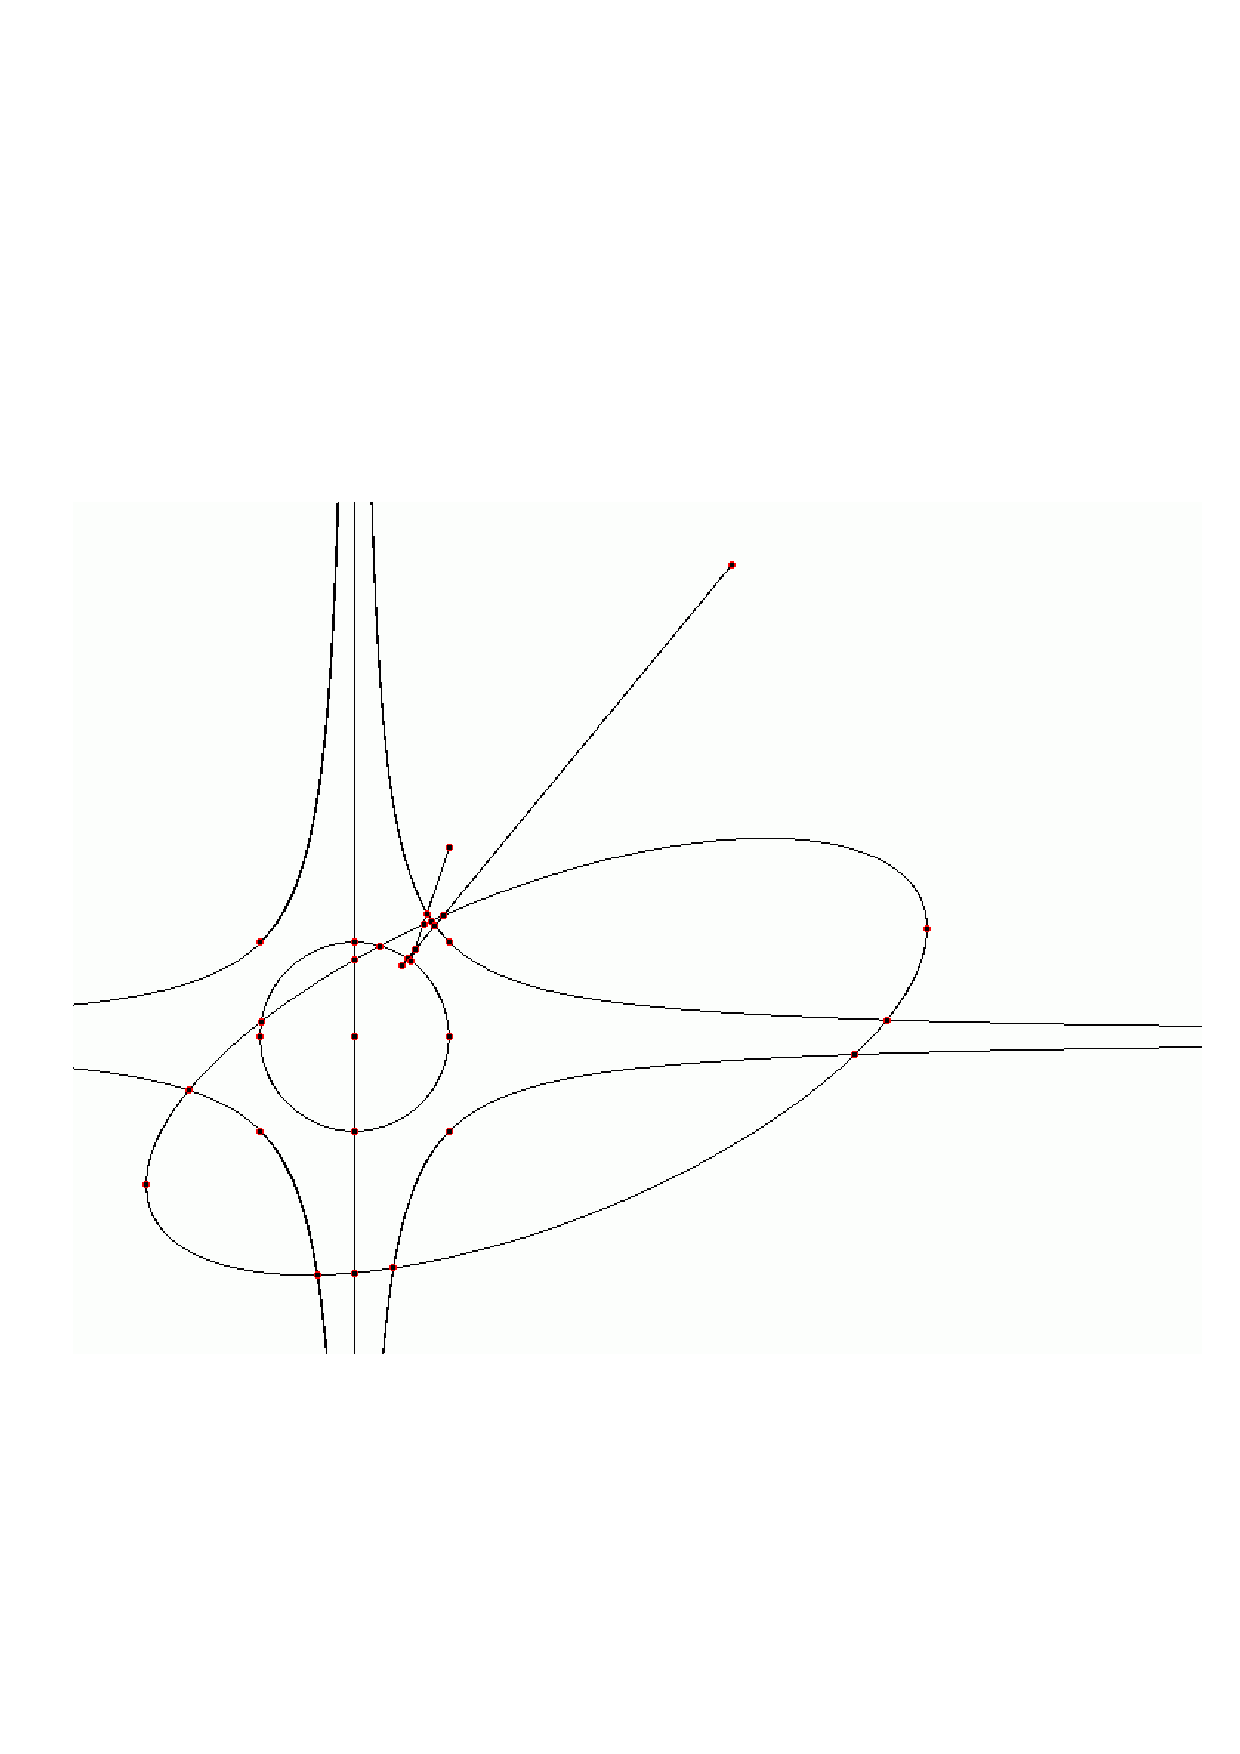
\includegraphics[width=0.7\textwidth]{Benchmark/fig/Conics_14_1}}
\end{ccTexOnly}
\begin{ccHtmlOnly}
  <p><center>
  <img src="./fig/Conics_14_1.gif" border=0 alt="conics">
  </center>
\end{ccHtmlOnly}
\caption{The curves and arcs contained in the example benchmark file.
  \label{fig:example}}
\end{figure}

We give a longer example containing 14 object of different types; line
segments, circles, conics, bounded and unbounded arcs of conics. See
Figure~\ref{fig:example} for their geometry.

% \begin{ccTexOnly}
% \IncludeVerbatim{Benchmark/Conics_14_1.arr}
% \end{ccTexOnly}

% \begin{ccHtmlOnly}
% \ccIncludeExampleCode{Benchmark/Conics_14_1.arr}
% \end{ccHtmlOnly}

% -------------------------------------------------------------------------
\subsection{Visitor Design Pattern for the Parser}
\label{visitor}

To ease the use of the parser, we provide a visitor interface,
following the visitor design pattern~\cite{cgal:ghjv-dpero-95}.  An
application would derive its own visitor from the
\texttt{Benchmark\_visitor} base class. This design choice makes the
parser independent of application types, such as long integers.
Instead, the parser keeps almost all recognized literals in strings of
type \texttt{std::string}.

The visitor has various functions that will be called from the parser
with suitable parameters when the parser recognizes certain grammar
rules. The visitor can then rely on the fact that the file is well
formed and just process the parameters. Typically the visitor will
store the objects found in the benchmark file in an internal data
structure for later use in the application. The visitor has to convert
the string parameters to the application specific types, for example,
for long integers for curve coefficients. 

\subsubsection{A First Visitor}
\label{checker}

We start with an example for a basic visitor that just checks a
benchmark file for correct syntax, i.e., it does not actually process
the objects in the file. Programs using the visitor will look similar,
but they will typically implement more member functions of the base
class interface, see Section~\ref{functions}. This example program
exists in source code in the distribution at
\verb|BMTools/parser/src/check_syntax.C|. 

\begin{verbatim}
#include <iostream>
#include <benchmark_visitor.hpp>

struct Checker : public Benchmark_visitor {
    Checker() {}
\end{verbatim}

\noindent
The visitor class \texttt{Checker} is derived from the
\texttt{Benchmark\_visitor} base class and has a default constructor.
The base class defines the interface for all visitors in terms of
virtual member functions that we can override in the derived class.
All member functions have sensible defaults that simplify the
implementation of a visitor that accepts only a subset of the objects.
For example, all object accepting member functions default to a call
to the error handler with a ``token not handled'' error message. We
explain in Section~\ref{functions} the available member functions and
in Section~\ref{extend} how the \texttt{Benchmark\_visitor} can be
extended. Here, we just override the particular error handler for 
the ``token not handled'' error message and disable the error message,
since we are just interested in accepting all tokens but do not handle
them individually.

\begin{verbatim}
    virtual void token_not_handled( std::string s) {}
\end{verbatim}

\noindent
In other typical visitor implementations this function would not be
overwritten because it is not called when the visitor recognizes and
processes a parameter properly. An example of such a processing is the
following handling of the  classification entries, which is handled
with the \texttt{classification} member function in the visitor that
accepts six string parameters for the different classification
entries. We implement a validness test that checks the parameters for
proper values.

\begin{verbatim}
    virtual void accept_classification( std::string problem,
                                        std::string geom, 
                                        std::string clas,
                                        std::string family,
                                        std::string instance,
                                        std::string release) {
        if ((problem != "Arrangement") && (problem != "CSG") 
            && (problem != " "))
            error_handler( "classification error");

        if ((geom != "Lines") && (geom != "Circles") && (geom != "Conics") 
            && (geom != "Cubics") && (geom != "Quartics") 
            && (geom != "ArbitraryDegreeCurves") && ( geom != "Quadrics") 
            && (geom != "Tori") && (geom != "Planes") && (geom != " "))
            error_handler( "classification error" );

        if ((clas != "FullCurves") && (clas != "Ellipses") 
            && (clas != "BoundedArcs") && (clas != "UnboundedArcs") 
            && (clas != "FullSurfaces") && (clas != "BoundedPatches")
            && (clas != "UnboundedPatches") && (clas != " "))
            error_handler( "classification error" );
    }
\end{verbatim}

\noindent
In addition, we use the benchmark name for a suitable diagnostic
output. For this, we override the implementation of the
\texttt{accept\_benchmark\_name} member function that accepts one
string parameters for the name. However, the base class implementation
of this function stores the name in the base class for later access
with the \texttt{benchmark\_name} member function, for example for
error messages, that we want to preserve. The easiest solution is to
call the implementation of the member function in the base class as
well. That finishes our visitor implementation.

\begin{verbatim}
    virtual void accept_benchmark_name( std::string s) {
        Benchmark_visitor::accept_benchmark_name(s);
        std::cerr << "name '" << s << "', ";
    }
};
\end{verbatim}

\noindent
It follows a simple main program that checks all files given by their
filenames on the command line for syntax errors and prints a suitable
diagnostic message.

\begin{verbatim}
int main( int argc, char* argv[] ) {
    int exit_status = 0;
    for ( int i = 1; i < argc; ++i) {
        Checker check;
        std::cerr << "File '" << argv[i] << "', ";
        if ( benchmark_parse_file( argv[i], & check)) {
            std::cerr << "is o.k." << std::endl;
        } else {
            std::cerr << "is malformed." << std::endl;
            exit_status = 1;
        }
    }
    return exit_status;
}
\end{verbatim}

\noindent
A similar global parser function allows parsing from an already opened
\CC\ stream. However, a stream is lacking useful diagnostic
information---filename and line number---that we provide explicitly
for this global parser function, where the line number has the
sensible default to start at one. Both functions return \texttt{true}
if the file parses without error, and \texttt{false} otherwise. The
full function signatures are:

\begin{verbatim}
bool benchmark_parse_file(   std::string name, Benchmark_visitor* v);
bool benchmark_parse_stream( std::istream&  in, std::string name, 
                             Benchmark_visitor* v, int n = 1);
\end{verbatim}


\subsubsection{Benchmark Visitor Functions}
\label{functions}

In the following table the functions that exist in the
\ccc{Benchmark_visitor} class are listed.  The \$-bison syntax
denotes the value of the arguments in the grammar rule, typically the
integer and strings, counting terminal symbols, non-terminal symbols,
and also the blocks in curly braces.  For their semantic specification
see Section~\ref{grammar} and Section~\ref{extend}.  The statements in
curly braces 
% \Open\ts{...}\Close\ 
\texttt{\{...\}}
are function calls to the visitor.
They come in two flavors, either a single function call, such as in
\texttt{accept\_integer(\$1)} for integers, if the entry has a small
constant number of parameters and only a few variants, or a pair of
functions that enclose the parsing of the parameters and form a proper
bracketing, such as for polynomials with
\ccc{begin_polynomial_1()} and \ccc{end_polynomial_1()},
where its integer coefficients are detected between these two function
calls. 

A typical visitor would maintain a list of integers, initialize
it in the \ccc{begin_polynomial_1()} call, stores all integers
accepted in the \ccc{accept_integer(\$1)} function in this list,
and builds a new polynomial from the list in the
\ccc{end_polynomial_1()} function. In general, a visitor
implementation would work with stacks to reflect the recursive nature
of the grammar.

\begin{ccTexOnly}
\begin{tabular}{*{2}{| l} |} \hline
Object   & grammar rule with visitor function          \\ \hline \hline
Integer  & {\bf Integer} \{accept\_integer(\$1);\}  \\ \hline
Rational & {\bf Rational ( Integer , Integer )} \{accept\_rational(\$3, \$5);\} \\ \hline
 Infty    & {\bf MINUS\_INFTY} \{accept\_infty(\$1);\}  \\ 
          & {\bf PLUS\_INFTY} \{accept\_infty(\$1);\}  \\ \hline
Orientation  & {\bf COUNTERCLOCKWISE} \\
             & {\bf CLOCKWISE} \\
             & {\bf VOID}          \\ \hline
Integer\_sequence &  {\bf Integer} \{accept\_integer(\$1);\} \\
                  & Integer\_sequence {\bf \Large ,} {\bf Integer} \{accept\_integer(\$3);\} \\ \hline
 Point\_2 & {\bf Point\_2 ( Integer , Integer )} \{accept\_point\_2(\$3, \$5);\} \\ 
          & {\bf Point\_2 ( Integer , Integer , Integer )} \{accept\_point\_2(\$3, \$5, \$7);\} \\
          & {\bf Point\_2 ( Rational ( Integer , Integer ) , Rational ( Integer , Integer ) )}\\
          & \ \ \ \ \{accept\_point\_2(\$5, \$7, \$12, \$14);\} \\ \hline
Polynomial &  {\bf Polynomial\_1} \{begin\_polynomial\_1();\} {\bf \Large (} Integer\_sequence {\bf \Large )}\\
           & \ \ \ \ \{end\_polynomial\_1();\} \\ \hline
AlgebraicReal & {\bf AlgebraicReal} \{begin\_algebraic\_real();\} {\bf \Large (}\\
              & \ \ {\bf Polynomial\_1} \{begin\_polynomial\_1();\}\\
              & \ \ \ \ \ {\bf \Large (} Integer\_sequence {\bf \Large )}\\
              & \ \ \ \ \ \ \ \ \ \{end\_polynomial\_1();\} {\bf \Large ,}         \\
              & \ \ Rational {\bf \Large ,} Rational {\bf \Large ,}  \\
              & \ \ {\bf Integer} \{accept\_integer(\$15);\} {\bf \Large )} \\
              & \ \ \ \ \{end\_algebraic\_real();\} \\ \hline          
LineSegment &  {\bf LineSegment\_2} \{begin\_line\_segment\_2();\} {\bf \Large (} Point\_2 {\bf \Large ,} \\
            & \ \ \ \ \ \ \ \ \ \  Point\_2 {\bf \Large )} \{end\_line\_segment\_2();\}\\ \hline
Circle   &  {\bf Circle\_2} \{begin\_circle\_2();\} {\bf \Large (} Point\_2 {\bf \Large ,} \\
         & {\bf Integer} \{accept\_integer(\$6);\} {\bf \Large )} \{end\_circle\_2();\} \\ 
Circle   &  {\bf Circle\_2} \{begin\_circle\_2();\} {\bf \Large (} Point\_2 {\bf \Large ,} Rational {\bf \Large )} \{end\_circle\_2();\} \\ \hline
Conic    & {\bf Conic\_2 ( Integer, Integer, Integer, Integer, Integer, Integer )} \\
              & \{accept\_conic\_2 (\$3, \$5, \$7, \$9, \$11, \$13);\}\\ \hline
ConicPoint    & {\bf ConicPoint\_2} \{begin\_conic\_point\_2();\} {\bf (} Conic ,            \\
              & \ \ AlgebraicReal {\bf \Large ,} Integer {\bf \Large )}  \\
              & \ \ \ \ \ \ \ \ \ \{end\_conic\_point\_2();\}\\ 
              & {\bf ConicPoint\_2} \{begin\_conic\_point\_2();\} {\bf (} Conic ,            \\
              & \ \ Infty {\bf \Large ,} Integer {\bf \Large )}  \\
              & \ \ \ \ \ \ \ \ \ \{end\_conic\_point\_2();\}\\ 
 & {\bf ConicPoint\_2} \{begin\_conic\_point\_2();\} {\bf (} Conic ,            \\
              & \ \ AlgebraicReal {\bf \Large ,} Infty {\bf \Large )}  \\
              & \ \ \ \ \ \ \ \ \ \{end\_conic\_point\_2();\}\\ \hline
ConicArc      & {\bf ConicArc\_2} \{begin\_conic\_arc\_2();\} {\bf \Large (} Conic {\bf \Large ,}   \\
              & \ \ ConicPoint {\bf \Large ,}                    \\
              & \ \ ConicPoint {\bf \Large ,}                    \\
              & \ \ orientation \{accept\_orientation(\$10);\} {\bf \Large )}                  \\
              & \{end\_conic\_arc\_2();\}\\
              & {\bf ConicArc\_2} \{begin\_conic\_arc\_2();\} {\bf \Large (} ConicPoint {\bf \Large )} \{end\_conic\_arc\_2();\}\\ \hline
Cubic   & {\bf Cubic\_2 (}        \\
        & \ \ {\bf Integer , Integer , Integer , Integer , Integer ,} \\
        & \ \ {\bf Integer , Integer , Integer , Integer , Integer )}  \\
        & \{accept\_cubic\_2 (\$3, \$5, \$7, \$9, \$11, \$13, \$15, \$17, \$19, \$21);\}\\ \hline
Quadric & {\bf Quadric\_3 (}      \\
        & \ \ {\bf Integer , Integer , Integer , Integer , Integer ,}  \\
        & \ \ {\bf Integer , Integer , Integer , Integer , Integer )}                  \\ 
        & \{accept\_quadric\_3 (\$3, \$5, \$7, \$9, \$11, \$13, \$15, \$17, \$19, \$21);\}\\ \hline
\end{tabular}
\end{ccTexOnly}

\begin{ccHtmlOnly}
<div align="center">
<table cellpadding=3 border="1">
<tr><th>Object</th><th>grammar rule with visitor function</th></tr>
</table>
</div>
\end{ccHtmlOnly}

% -------------------------------------------------------------------------
\subsection{Extending the Parser}
\label{extendall}

We describe the key changes necessary to add new tokens and new rules
to the parser. We assume, we want to a add a new element \texttt{Foo}
that needs a \texttt{double} value and an \texttt{integer} value.

\subsubsection{Extend the Scanner in \texttt{benchmark\_lexer.l}}

We jump to a section with the word \texttt{Token} in a comment. It
looks about like this:

\begin{verbatim}
 /* Tokens    */
 /* --------- */
"FileFormat"                    { return FileFormat;}
"BenchmarkName"                 { return BenchmarkName; }
"List"                          { return List;}
"Rational"                      { return Rational;}
\end{verbatim}

\noindent
and several more lines like this. And we add our new element as own
line anywhere in this section, like:

\begin{verbatim}
"Foo"                           { return Foo;}
\end{verbatim}

\noindent
Note that the left \texttt{"Foo"} and the right \texttt{Foo} do not
have to be the same word, the left string is the representation in the
file format, the right word is its identifier in the program code. We
use the same word though for simplicity.

\subsubsection{Extend the Parser in \texttt{benchmark\_parser.y}}
\label{extend}
We jump to the section with the words \texttt{Header tokens} in a
comment. It looks about like this:

\begin{verbatim}
/* Structure tokens */
/* ---------------- */
%token FileFormat
%token BenchmarkName
%token List
%token Rational
\end{verbatim}

\noindent
and add our new token anywhere in this block like this:

\begin{verbatim}
%token Foo
\end{verbatim}

\noindent
We continue and add new rules in the grammar section. Two common
choices are most likely: Either, the new token has a constant number
of (or only a few optional) parameters or the new token allows a
variable list of arguments. For the former case, we add one rule
including all arguments and call a single new function in the visitor;
see the rule for \texttt{Rational(...)} as an example. We also have to
decide, in which part of the grammar we like the new token to be
accepted. Likely places for extensions are \texttt{stmt} or
\texttt{file\_header\_option}. We add our rule example for
\texttt{Foo} in the \texttt{stmt} block right after the
\texttt{Rational} rule:

\begin{verbatim}
  | Foo '(' double_val ',' INTEGER ')'
                        { visitor->accept_foo( atof( $3.c_str(), $5); }
\end{verbatim}

\noindent
The parameters are enclosed in parenthesis and separated with
commas. The double value could be either an \texttt{INTEGER} or an
\texttt{FNUMBER}, so we use the production \texttt{double\_val} that
accepts both. Its return type is a \texttt{std::string} denoted with
\texttt{\$3} that contains the number representation. We use the
\texttt{atof()} function to simplify the work for the visitor. We
could do the same for the \texttt{INTEGER} parameter in \texttt{\$5}
if we would expect some small bounded integer, but for unbounded long
integer numbers we pass the original \texttt{std::string} and let the
visitor do the conversion in the long integer type that is only known
to the application.

Now let us assume we would like to have \texttt{Foo} with a variable
parameter list of arguments. We add one rule with a production
referring to the variable list of arguments and call a new function
of the visitor before we enter this variable length production  and we call a 
second new function of the visitor at the end of the variable length
production; see the rule for \texttt{Polynomial\_1(...)} as an example.
We add the rule again in the \texttt{stmt} production.

\begin{verbatim}
  | Foo                { visitor->begin_foo(); }
       '(' integer_sequence ')' { visitor->end_foo(); }
\end{verbatim}

\noindent
So, the \texttt{begin\_foo} function is called before the integers are
parsed, and once all integers are parsed (and the corresponding
function \texttt{accept\_integer} has been called for each integer) the
function \texttt{end\_foo} is called, effectively creating a proper
bracketing structure around the integer sequence.

\subsubsection{Extend the Visitor in \texttt{benchmark\_visitor.h}}
The visitor follows the visitor design pattern in
~\cite{cgal:ghjv-dpero-95}, see Section~\ref{visitor}.
Depending on the two options in the previous section we have to add to
the \texttt{Benchmark\_visitor} class a member function

\begin{verbatim}
    virtual void accept_foo( double d, std::string i) { tnh( "Foo"); }
\end{verbatim}

\noindent
or two member functions

\begin{verbatim}
    virtual void begin_foo() { tnh( "Begin_foo"); }
    virtual void end_foo()   { tnh( "End_foo"); }
\end{verbatim}

\noindent
We implement these member functions with calls to the \texttt{tnh}
function, which is a short-cut for the \texttt{token\_not\_handled}
member function that issues by default an error message about an
un-handled token. So, a derived visitor class that does not override
these virtual \texttt{foo} functions still works fine on files that do
not have any \texttt{Foo} in them, but they will generate error
messages by default. This can be suppressed, see the \texttt{check\_syntax}
example program for an useful application in Chapter~\ref{checker}.


\section{Execution}
This section lists the various command-line options a benchmark
program may accepts, and it explains how to create a hierarchy of
programs and execute the programs in the hierarchy selectively using
an agent implemented in \textbf{Perl}.

Some pieces of the toolkits are dedicated to the development and
maintenance of the \cgal\ planar map modules. For example, some of
the command-line options listed below directly control the behavior
of the planar-map benchmarks, and it's hard to imagine how they can be
applied to other benchmarks. While these pieces should be
reimplemented or even removed all together, in order to make the
toolkit fully generic, other users may ignore them for the time being.

\subsection{Command-Line Options}
A program written with the aid of the \ccc{Bench_option_parser}
class accepts the command-line options listed below. The command-line options
must be provided after the executable name and before an optional name of an
input file. A brief description is displayed on the console as a
response to the \textbf{`` -h''} option.

\begin{list}{}
  {
    \setlength{\topsep}{0pt}
    \setlength{\partopsep}{0pt}
    \setlength{\parskip}{0pt}
    \setlength{\parsep}{0pt}
    \setlength{\itemsep}{0pt}
    \setlength{\itemindent}{0pt}
    \setlength{\leftmargin}{0.2\textwidth}
    \setlength{\labelsep}{0pt}
    \setlength{\labelwidth}{0.2\textwidth}
    \settowidth{\listparindent}{abc}
  }
\item[\bf{-b {\em options}}\hfill]
  set bench options

  \begin{list}{}
    {
      \setlength{\topsep}{0pt}
      \setlength{\partopsep}{0pt}
      \setlength{\parskip}{0pt}
      \setlength{\parsep}{0pt}
      \setlength{\itemsep}{0pt}
      \setlength{\itemindent}{0pt}
      \setlength{\leftmargin}{0.2\textwidth}
      \setlength{\labelsep}{0pt}
      \setlength{\labelwidth}{0.2\textwidth}
      \settowidth{\listparindent}{abc}
    }
  \item[\bf{type\_name={\em type}}\hfill]
  \item[\bf{tn={\em type}}\hfill]
    set bench type to {\em type} (default all).\\
    {\em type} is one of:
    \begin{list}{}
      {
	\setlength{\topsep}{0pt}
	\setlength{\partopsep}{0pt}
	\setlength{\parskip}{0pt}
	\setlength{\parsep}{0pt}
	\setlength{\itemsep}{0pt}
	\setlength{\itemindent}{0pt}
	\setlength{\leftmargin}{0.2\textwidth}
	\setlength{\labelsep}{0pt}
	\setlength{\labelwidth}{0.2\textwidth}
	\settowidth{\listparindent}{abc}
      }
    \item[\bf{i[ncrement]}\hfill] \bf{0x1}
    \item[\bf{a[ggregate]}\hfill] \bf{0x2}
    \item[\bf{d[isplay]}\hfill] \bf{0x4}
    \end{list}
  \item[\bf{type\_mask={\em mask}}\hfill]
  \item[\bf{tm={\em mask}}\hfill]
    set bench type mask to {\em mask}
  \item[\bf{strategy\_name={\em strategy}}\hfill]
  \item[\bf{sn={\em strategy}}\hfill]
    set bench strategy to {\em strategy} (default all).\\
    {\em strategy} is one of:
    \begin{list}{}
      {
	\setlength{\topsep}{0pt}
	\setlength{\partopsep}{0pt}
	\setlength{\parskip}{0pt}
	\setlength{\parsep}{0pt}
	\setlength{\itemsep}{0pt}
	\setlength{\itemindent}{0pt}
	\setlength{\leftmargin}{0.2\textwidth}
	\setlength{\labelsep}{0pt}
	\setlength{\labelwidth}{0.2\textwidth}
	\settowidth{\listparindent}{abcdefg}
      }
    \item[\bf{t[rapezoidal]}\hfill] \bf{0x1}
    \item[\bf{n[aive]}\hfill]       \bf{0x2}
    \item[\bf{w[alk]}\hfill]        \bf{0x4}
    \item[\bf{d[ummy]}\hfill]       \bf{0x8}
    \end{list}
  \item[\bf{strategy\_mask={\em mask}}\hfill]
  \item[\bf{sm={\em mask}}\hfill]\
    set bench strategy mask to {\em mask}
  \item[\bf{h[eader]={\em bool}}\hfill]
    print header (default \textbf{true})
  \item[\bf{name\_length={\em length}}\hfill]
  \item[\bf{nl={\em length}}\hfill]
    set the length of the name field to {\em length}
  \end{list}
\item[\bf{-d {\em dir}}\hfill]
  add directory {\em dir} to list of search directories
\item[\bf{-h}\hfill]
  print this help message
\item[\bf{-i {\em iters}}\hfill]
  set number of iterations to {\em iters} (default 0)
\item[\bf{-I {\em options}}\hfill]
  set input options
  \begin{list}{}
    {
      \setlength{\topsep}{0pt}
      \setlength{\partopsep}{0pt}
      \setlength{\parskip}{0pt}
      \setlength{\parsep}{0pt}
      \setlength{\itemsep}{0pt}
      \setlength{\itemindent}{0pt}
      \setlength{\leftmargin}{0.2\textwidth}
      \setlength{\labelsep}{0pt}
      \setlength{\labelwidth}{0.2\textwidth}
      \settowidth{\listparindent}{abcdefg}
    }
    \item[\bf{f[ormat]={\em format}}\hfill]
      set format to {\em format} (default \textbf{rat}).\\
      {\em format} is one of:
      \begin{list}{}
	{
	  \setlength{\topsep}{0pt}
	  \setlength{\partopsep}{0pt}
	  \setlength{\parskip}{0pt}
	  \setlength{\parsep}{0pt}
	  \setlength{\itemsep}{0pt}
	  \setlength{\itemindent}{0pt}
	  \setlength{\leftmargin}{0.2\textwidth}
	  \setlength{\labelsep}{0pt}
	  \setlength{\labelwidth}{0.2\textwidth}
	  \settowidth{\listparindent}{abcdefg}
	}
	\item[\bf{i[nt]}\hfill] integer
	\item[\bf{f[lt]}\hfill] floating point
	\item[\bf{r[at]}\hfill] rational
      \end{list}
  \end{list}
\item[\bf{-r {\em root}}\hfill]
  set the {\tt \$ROOT} to {\em root} (default is the environment
  variable {\tt \$ROOT})
\item[\bf{-s {\em samples}}\hfill]
  set number of samples to {\em samples} (default 10)
\item[\bf{-t {\em seconds}}\hfill]
  set number of seconds to {\em seconds} (default 1)
\item[\bf{-v}\hfill]
  toggle verbosity (default \textbf{false})
\end{list}

\subsubsection{Input}
The sole input file, if provided, must appear after the last
command-line option in the command line. This file is searched for in
a directory search-list. The initial list consists of the current
directory followed by {\tt \$ROOT/data/Segments\_2},
{\tt \$ROOT/data/Conics\_2}, and {\tt \$ROOT/data/Polylines\_2} in
this order, where {\tt \$ROOT} is initialized with the value of the
environment variable {\tt \$ROOT}, and possibly overridden using the
command line \textbf{``-r {\em root}''}

The \textbf{``-d {\em dir}''} command-line option inserts the
directory \textbf{\em dir} at the end of the search list.

We are aware to the need to extend the command-line parsing to handle
multiple input files. In addition the dedicated names
{\tt Segments\_2}, {\tt Conics\_2}, and {\tt Polylines\_2} should be
removed or extended.

The \ccc{get_input_format()} method of the
\ccc{Bench_option_parser} class returns the format provided
by the user through the \textbf{``-I format={\em format}''} command
line option, or \textbf{``-I f={\em format}''} in short.

\subsubsection{Output}
The output produced by a single benchmark program exemplified in
figure \ref{sqrtResults} is a text-based table easily readable by
humans. It consists of an optional header record and a data
record. The production of the header can be suppressed by the
\textbf{''-b header=false''} command-line option, or
\textbf{''-b h=false''} in short. Occasionally a sequence of
benchmarks are performed in a raw and the display of the header is
desired only once (or once per page).

A data record consists of the following fields:
\begin{description}
\item[Bench Name] the name of the benchmark.
\item[Bench Time] the allocated time-slot for the entire benchmark in
seconds (see \textbf{``-t {\em seconds}``} option).
\item[Ops Num] the number of target operations performed within the
time slot.
\item[Total Ops Time] the time required to perform the loop of
operations consisting of \textbf{Ops Num} operations in seconds.
\item[Single Op Time] the average time required to perform a single
operation in seconds.
\item[Num Ops Per Second] the number of operations completed per second.
\end{description}

The \textbf{Bench Name} field identifies the benchmark for all
purposes, its length is 32 characters by default. The length can
overridden by the \textbf{``-b name\_length={\em length}''}
command-line option, or \textbf{``-b nl={\em length}''} in short.

Independent tools listed in section \ref{Analysis} parse log files
that contain benchmark results, manipulate them, analyze them, and
perhaps convert them to other formats for artful presentations.

\subsection{Execution of multiple benchmarks}
The \textbf{Perl} script \textbf{cgal\_bench} selectively executes
multiple benchmarks ordered in a hierarchy. It executes them in a
sequence one at a time passing the appropriate command-line
options and input data file for each execution. It accepts a few
command-line options on its own listed below, and reads an input file
that contains the hierarchy of the benchmarks along with necessary
data required to execute them. This information is represented in a
simple language derived from the Extensible Markup Language (XML).

\subsubsection{Command-line options}

\begin{list}{}
  {
    \setlength{\topsep}{0pt}
    \setlength{\partopsep}{0pt}
    \setlength{\parskip}{0pt}
    \setlength{\parsep}{0pt}
    \setlength{\itemsep}{0pt}
    \setlength{\itemindent}{0pt}
    \setlength{\leftmargin}{0.2\textwidth}
    \setlength{\labelsep}{0pt}
    \setlength{\labelwidth}{0.2\textwidth}
    \settowidth{\listparindent}{abc}
  }
\item[\textbf{ -args {\em args}}\hfill]
  set additional arguments passed to the benchmark programs.
\item[\textbf{-help}\hfill]  
  print this help message.
\item[\textbf{-verbose {\em level}}\hfill]  
  set verbose level to \textbf{\em level} (default 0).
\item[\textbf{-database {\em file}}\hfill]  
  set database xml file to \textbf{\em file} (default
  {\tt \$ROOT/bench/data/benchDb.xml}).
\item[\textbf{-filter {\em name}}\hfill]  
  select bench \textbf{\em name}, and sub benches (default all).
\end{list}
  
A unique prefix is sufficient to indicate the desired
option. For example, when the \textbf{``-help''} option is specified, 
a brief description is displayed on the console, and the script quits
immediately after. The same behavior is achieved through the
abbreviated \textbf{``-hel''}, \textbf{``-he''}, and \textbf{``-h''}
options.

By default the script reads the file
{\tt \$ROOT/bench/data/benchDb.xml}. This can be overridden through
the \textbf{``-database {\em file}''} command-line option.

\subsubsection{Documenting the Environment}
The scripts automatically documents the environment in which it
performs the benchmarks, so the benchmark can be easily rerun
(provided the same environment is still available) and the 
results can be more accurately compared to the results of other
benchmarks.

The scripts extract most of the information directly from the
environment. Additional configuration data that cannot be extracted
directly from the environment is extracted from the  database input
file. The script prints out its finding, and only then it starts
performing the benchmarks. Here is an excerpt from a sample run of
{\tt cgal\_bench}, showing the type of information extracted and
printed out.

\begin{verbatim}
Mon Mar 31 20:29:02 2003
COMPILER NAME: gcc
COMPILER INFO: gcc (GCC) 3.2
Copyright (C) 2002 Free Software Foundation, Inc.
This is free software; see the source for copying conditions.  There is NO
warranty; not even for MERCHANTABILITY or FITNESS FOR A PARTICULAR PURPOSE.

OS NAME: linux
OS INFO: Linux cgal 2.4.20-net1 #1 SMP Wed Feb 5 13:05:52 IST 2003 i686 unknown

PROCESSOR: 0
CPU SPEED: 999.783 MHz
CPU TYPE: Pentium III (Coppermine)
PRIMARY DATA CACHE: 256 KB
SECONDARY DATA CACHE: 0
INSTRUCTION CACHE: 0
PROCESSOR: 1
CPU SPEED: 999.783 MHz
CPU TYPE: Pentium III (Coppermine)
PRIMARY DATA CACHE: 256 KB
SECONDARY DATA CACHE: 0
INSTRUCTION CACHE: 0
MEM SIZE: 2020 MBytes
GFX BOARD: unknown
CGAL VERSION: 2.5-I-81
LEDA VERSION: 441
QT VERSION: unknown
\end{verbatim}

\subsubsection{Input File Format}
The representation of the input file is derived from XML. Its element
tag-set consists of 4 predefined element tags listed below. All other
element tags that appear in an input file without exception are names
of executables that perform benchmarks.

The following is a list of the 4 elements with the 4 predefined tags
respectively:
\begin{description}
\item[file] specifies a file.
\item[bench] specifies a hierarchy of benchmarks.
\item[clo] specifies a command-line option.
\item[class] specifies a style-sheet class.
\end{description}

A \textbf{file} element specifies a data file provided as input to a
benchmark. It may have the following attributes:
\begin{description}
\item[name] - the file name.
\item[format] - the number type.
\item[curves] - the number of curves.
\item[vertices] - the number of vertices.
\item[halfedges] - the number of halfedges.
\item[faces] - the number of faces.
\end{description}

The \textbf{name} attribute is mandatory, as it identifies the file
for all purposes. The other attributes are optional (as a matter of
fact, the last 4 attributes are specific to the planar-map benchmarks.)

A \textbf{clo} element specifies a command-line option. It has the
following two mandatory attributes:
\begin{description}
\item[name] - the option name.
\item[string] - the option string.
\end{description}

The option name identifies the option for all purposes. The option
string is the exact argument that must appear in the command line for
that option to take effect.

A \textbf{bench} element specifies a hierarchy of benchmarks. It can
contain multiple \textbf{file}, \textbf{clo}, or \textbf{class}
elements, multiple elements that represent executables, and multiple
nested \textbf{bench} elements. The \textbf{file} attribute of a
\textbf{bench} element, if present, specifies an input data file. The
value of the \textbf{file} attribute is the name of the input file
(and the value of the \textbf{name} attributes of a \textbf{file}
element). Each attribute of a \textbf{bench} element that is neither
\textbf{file} nor \textbf{enable} specifies a command-line option. The
value of such an attribute is the option variable-value or
parameter. Command-line options are passed through inheritance in the
benchmark hierarchy, where an option parameter specified in a
\textbf{bench} element overrides the parameter specified higher in the
hierarchy. The boolean attribute \textbf{enable} simply indicates
whether the bench hierarchy should be executed or not.

The tag of a benchmark element is the name of an executable that
performs a benchmark. A benchmark element, just like a \textbf{bench}
element, may contain a \textbf{file} attribute to indicate an input
data file, a \textbf{enable} attribute to enable or disable the
benchmark, and multiple attributes, each indicating the parameter of a
command-line option.

A \textbf{class} element is used only while generating files for
browsing (e.g., html, php, etc.). 

Figure \ref{database} lists a simple bench input-file that consists
of three benchmarks, three corresponding input files, and some
command-line options that are used to execute the benchmarks. When
this file is provided as input to the \textbf{cgal\_bench} script, the
later parses the file, interprets its contents, and executes the
commands below in turn:
\begin{verbatim}
bench1 -s 10 -bh=true -bnl=64 file1
bench2 -s 10 -bh=flase -bnl=64 file2
bench3 -s 10 -bh=flase -bnl=64 file3
\end{verbatim}

\begin{figure}[!hbp]
\begin{fminipage}{\textwidth}
\begin{alltt}
<?xml version="1.0" encoding="ISO-8859-1"?>
<\textbf{\Red{bench}} name_length="64" header="false">
  <\textbf{\GREEN{clo}} name="samples" string="-s"/>
  <\textbf{\GREEN{clo}} name="name_length" string="-bnl="/> 
  <\textbf{\GREEN{clo}} name="header" string="-bh="/> 
  <\textbf{\GREEN{clo}} name="format" string="-If="/>

  <\textbf{\GBLUE{file}} name="file1" format="rat"/>
  <\textbf{\GBLUE{file}} name="file2" format="rat"/>
  <\textbf{\GBLUE{file}} name="file3" format="rat"/>

  <\textbf{\Red{bench}} samples="10" enable="true">
    <\textbf{\Red{bench1}} file="file1" header="true"/>
    <\textbf{\Maroon{bench2}} file="file2"/>
    <\textbf{\Apricot{bench2}} file="file3"/>
  </bench>
</bench>  
\end{alltt}
\end{fminipage}
\caption{A simple database}\label{database}
\end{figure}

\section{Analysis\label{Analysis}}
The scripts in this category are intended to analyse and profile
results of benchmarks and convert the resulting data into more
meaningful and comprehensible presentations. They parse log files that
contain benchmark results, interpret the data, manipulate it, analyze
it, and perhaps convert it into other formats for artful presentations.

In principle they should be able to 1. add new fields to the
predefined fields of a benchmark data-record. This can be useful to
perform mathematical operations on the data values, or to reformat the
output for pretty printing, 2. merge records, 3. sort the records, 
4. filter out records, and 5. convert the data into other formats.

Converting the textual results into other formats that support artful
presentations, pretty printing, and browsing capabilities is
deficient, as this part of the toolkit consists of a single
{\textbf Perl} script that converts benchmark results into a dedicated
php script that can be quickly integrated into the Tel-Aviv local
\cgal\ web site (not very useful for other users).

The \textbf{bash} command-line below can be used to record benchmark
results in separate log files in the {\tt \~{}/logs} directory:
 
\begin{verbatim}
cgal_bench <flags> 2>&1 | tee ~/logs/bcgal_`date +%y%m%d%%%H%M%S`.log
\end{verbatim}

When these log files are sorted by name, which is typically the
default, it is fairly easy to point at the most recent log file.

\section{Leftturn example}
The following example measures the performance of the left-turn predicate
in \cgal.
\ccIncludeExampleCode{../examples/Benchmark/leftturn.cpp}

The result
\begin{verbatim}
Bench                            Bench    Ops      Total    Single   Num Ops
    Name                             Time      Num Ops Time  Op Time  Per Sec
-------------------------------- -------- -------- -------- -------- --------
Leftturn                                1    90242   0.9900   0.0000 91153.5345
\end{verbatim}

\section{Acknowledgement}
The benchmark file-format and the reference parser implementation was 
developed at Max-Planck-Institut f\"ur Informatik, Saarbr\"ucken, Germany, by
Eric Berberich, Franziska Ebert, and Lutz Kettner as part of the 
\textsc{Acs} project.
 

% conforms to the
% test agent
% performance profiling
% ------------------------------------------
% Automatic tests are arranged in a hierarchy. A set of super-tests comprises the highest level. Each super-test consists of a group of sub-tests that have something in common. For example, they all test X3D IndexedfaceSet features. Each sub-test is associated with an *.html file. The tests are executed sequentially. For each super-test, the browser is run from the command line. When the agent (script) that runs the browser, detects that the last sub-test within the current super has completed, it submits a kill signal that terminates the browser. For each sub-test the associated html file is loaded onto the browser from the command line. When the agent detects that the sub-test has terminated, it analyzes the test output to determine whether the test failed or succeeded. Next, the html associated with the next sub-test is loaded. These steps are repeated until all super-tests are run. The entire process is repeated for various configurations.
% ------------------------------------------
% 1 : the act or an instance of regressing
% 2 : a trend or shift toward a lower or less perfect state: as a :
% progressive decline of a manifestation of disease b (1) : gradual loss
% of differentiation and function by a body part especially as a
% physiological change accompanying aging (2) : gradual loss of memories
% and acquired skills c : reversion to an earlier mental or behavioral
% level d : a functional relationship between two or more correlated
% variables that is often empirically determined from data and is used
% especially to predict values of one variable when given values of the
% others <the regression of y on x is linear>; specifically : a function
% that yields the mean value of a random variable under the condition
% that one or more independent variables have specified values 
% 3 : retrograde motion
% ------------------------------------------
% <benchmark> A standard program or set of programs which can be run on
% different computers to give an inaccurate measure of their
% performance. 
% 
% "In the computer industry, there are three kinds of lies: lies, damn
% lies, and benchmarks." 
% 
% A benchmark may attempt to indicate the overall power of a system by
% including a "typical" mixture of programs or it may attempt to measure
% more specific aspects of performance, like graphics, I/O or
% computation (integer or floating-point). Others measure specific tasks
% like rendering polygons, reading and writing files or performing
% operations on matrices. The most useful kind of benchmark is one which
% is tailored to a user's own typical tasks. While no one benchmark can
% fully characterize overall system performance, the results of a
% variety of realistic benchmarks can give valuable insight into
% expected real performance. 
% 
% Benchmarks should be carefully interpreted, you should know exactly
% which benchmark was run (name, version); exactly what configuration
% was it run on (CPU, memory, compiler options, single user/multi-user,
% peripherals, network); how does the benchmark relate to your workload? 
% 
% Well-known benchmarks include Whetstone, Dhrystone, Rhealstone (see
% h), the Gabriel benchmarks for Lisp, the SPECmark suite, and
% LINPACK. 
